\appendix
\chapter{Coordinates, Signals, and Reproduction}
\label{chap:appendix}
\label{app:signals}

\section{Pose and Force Signal Definitions}
The position vector is expressed in millimeters and orientation as a rotation vector in radians. The matrix \(R=\operatorname{Exp}([\rho]_\times)\) maps a vector in the calibrated tool frame to the robot base when it represents \(R_{B\leftarrow E}\). \([\rho]_\times\) is the skew-symmetric matrix associated with \(\rho\). The saved dataset transformation subtracts only \((c_x,c_y)\). The optional inference transformation additionally rotates center-relative XY by \(R_2(\alpha)\), with inverse rotation followed by center addition on output (Section~\ref{sec:stain_relative_generalization}). Both retain Z, tool rotation vectors, and force channels. The evaluated E1/E2 settings use \(\alpha=0\).

Teaching force is a three-component post-publisher measurement. Its associated tool orientation supplies the base-axis rotation in Equation~\eqref{eq:normal_force_projection}. Robot wrench feedback is already base expressed. A torque reference-point transformation would require a moment arm, but no torque transfer is needed for the three-force-component base projection used here. The available analysis does not infer a calibrated compliant contact point from a TCP-center trajectory.

Table~\ref{tab:force_roles} distinguishes the force signal roles.

\begin{table}[tbp]\centering\small
\caption[Force signal definitions]{Force signal roles used throughout the thesis.}
\label{tab:force_roles}
\begin{tabularx}{\textwidth}{P{0.31\textwidth}X}
\toprule Signal & Interpretation \\ \midrule
Teaching intention & Operator's approximate loading intention; not a numeric command trace. \\
Teaching recorded force & Measured interaction after the published processing path; used to construct learning supervision. \\
Policy force action & Denormalized output of the generator before executor gating and slew. \\
Executor transmitted target & Command-side force after shared processing; tangential target channels disabled in these comparisons. \\
Controller-applied reference & Target after internal controller processing; synchronized trace unavailable. \\
Robot measured force & Processed base-frame feedback used by the common gate, policy adapter, and recorded analysis. \\
\bottomrule
\end{tabularx}
\end{table}

\section{Learning and Temporal Parameters}
The force-cleanup dataset contains 15,963 paired frames in 42 compact episodes. The optimization and validation sets contain 38 and four episodes. Validation episode identifiers are 35, 39, 22, and 37. Each epoch's training window construction uses 50 starts per episode, a 128-step target, and the archived phase-sampling weights. The partition stored in each normalizer matches the dataset manifest.

The force-history dimension is three, its sample count is 30, and the selected recurrent layer is a one-layer GRU with hidden size 64. The state encoder receives pose and current force together in B/C. A removes the force state dimensions and history encoder. B retains the history architecture with zeroed conditioning. Physical force remains available to common execution in all conditions.

The training horizon, reference stride, inference timer, command period, and logging cap describe different mechanisms:
\begin{table}[tbp]\centering\small
\caption[Distinct clocks and sampling settings]{Distinct clocks and sampling settings.}
\label{tab:clock_definitions}
\begin{tabularx}{\textwidth}{P{0.39\textwidth}X}
\toprule Mechanism & Value or meaning \\ \midrule
Teaching paired sample grid & Nominal 30 Hz; original receipt times retained in merged HDF5. \\
Action sequence & 128 samples, nominal 30 Hz. \\
Nominal new-plan stride & 120 action samples at 30 Hz: 4.0 s. \\
E3 replanning lead / plan-age threshold & 0.5 s / \(4.0-0.5=3.5\) s, from saved configurations and runtime snapshot. \\
Actual plan-generation intervals & Not measured here; affected by callback scheduling and inference latency. \\
Inference callback timer & 5 Hz, subject to plan-age gating. \\
Flow integration & 10 dimensionless updates per generated chunk. \\
Command publication & Nominal 125 Hz (0.008 s). \\
E1 actual receipt-event recording & Approximately 125 Hz in the 15 October primary cohort; distinct subscription receipts. \\
E2 feedback CSV logging & 20 Hz cap; approximately 18 Hz observed in the 13 October archive. \\
Analysis support & Receipt-time ZOH force and within-support pose interpolation; maximum gap 0.2 s. \\
\bottomrule
\end{tabularx}
\end{table}

\section{Data and Analysis Reproducibility}
The run-level results retain the original identifiers, cohort membership, saved configurations, and analysis definitions. E1/E2 statistics use the archived precision CSVs matched to their frozen selections. E1's additional \(R^{*}\) cohort preserves its separate collection and unrounded values. The common result summary supplies the numerical tables and reported aggregates.

E3 reproduction uses the original before/after RGB hashes, saved visible-boundary annotations, fixed ROI construction, and archived segmentation algorithm. The reproduced initial/final ink masks and ROI arrays agree pixel by pixel with the stored analysis outputs. The displayed photographs and binary masks remain distinct from conceptual diagrams and from uncalibrated execution heatmaps. Display cropping and enlargement never supply the measured areas.

The accompanying analysis manifests identify the source inputs, per-run configuration and image mapping, numerical precision, and software versions. Document construction uses the bundled figures, selected original photographs, bibliography, and LaTeX sources. Repeating the full image analysis additionally requires the original research archive. Both procedures preserve the recorded sample selection and unavailable measurements.

\chapter{Experiment Versions and Provenance}
\label{app:provenance}

\section{Selected Models and Dataset}
The dataset and models are the force-cleanup revision dated 12 October, with training completed on 13 October 2026. All three selected checkpoints have their own normalizer. The best epochs are 39, 42, and 42, while final epoch is 499. The stored checkpoint selection rule is minimum validation loss over 500 epochs. The model manifest preserves the original CPU metadata inspection. The E3 C checkpoint and normalizer files also match the hashes in every selected execution configuration; they are hashed without model loading or retraining.

Table~\ref{tab:model_provenance} lists the selected model identifiers.

\begin{table}[tbp]\centering\small
\caption[Selected model identifiers]{Short SHA-256 identifiers of the selected checkpoints and normalizers. Complete values are included in the supplied model manifest.}
\label{tab:model_provenance}
\begin{tabular}{lll}
\toprule Model & Checkpoint prefix & Normalizer prefix \\ \midrule
A & \texttt{2ea204ab65fb} & \texttt{ae7d07adf65a} \\
B & \texttt{080103e6c2ed} & \texttt{d7c917b8246c} \\
C & \texttt{60d55e7092cb} & \texttt{09111fa4acc3} \\
\bottomrule
\end{tabular}
\end{table}

The compact replay episode is linked to the source merged HDF5 recorded at 16:18 on 19 August 2026, source episode \texttt{ep\_0003}. Its compact action and observation pose/force arrays contain 443 frames. The original source-time array is retained for T rather than replaced by an assumed constant period. The exact source paths and extraction fields are recorded in the supplied episode metadata.

\section{Primary E1 Version and Membership}
The physically executed primary cohort is
\begin{quote}\small\path{E1_CT_pass_height_v2_nominal_dev_20261015}\end{quote}
with configuration \texttt{e1ct\_46de718a23a2a7cf}, evaluator \texttt{pass\_height\_ref\_v2}, and observer \texttt{received\_observations\_v2}. The source report freezes the 15 planned run identifiers. Each planned slot has one started primary execution, and the original C5 remains the run ending in \texttt{230120\_b45d2f021b}. Its full identifier and the additional C6 identifier are recorded in the cohort manifest.

C6 is the later execution ending in \texttt{233551\_9021584d0a}. It retains repeat index 5 and the source retry link in the original archive, but is displayed as C6 for diagnostic interpretation. The subsequent session list therefore has 16 entries, while the primary E1 set remains the report-frozen 15. The explicit selection uses planned slots and original identifiers rather than the most recent record per repeated index. The same C checkpoint and frozen execution setting are retained.

The handoff \path{baseline_manifest.json} still contains preparation-era zero-attempt fields. The actual report, original execution evidence, and frozen report membership supersede those status fields for this thesis. The nominal placement is operator reported; the configured approximate surface Z is not a per-trial physical measurement. LOW/HIGH and reference-offset robustness are outside the completed evaluation scope.

\section{Historical E1 Development and Height-Only Replay}
\label{app:e1_history}
The 14 October development session, \texttt{E1\_CT\_sync\_confirm\_dev\_20261014}, uses configuration \texttt{e1ct\_61a19f7d7337a82c} and the initial-contact height reference. Its started order is R, then T, then C. All 15 started runs show the required loaded pass, while the old exit criterion reports R 3/5, T 4/5, and C 5/5. Table~\ref{tab:e1_historical_primary} preserves this historical comparison separately from the primary 15 October results.

\begin{table}[tbp]\centering\footnotesize
\caption[Historical 14 October E1 results]{Historical 14 October E1 development cohort with the initial-contact height reference. Completed-time means use \(n=3,4,5\) for R/T/C; excess-force summaries retain five started runs per method. These executions are not pooled with the primary cohort.}
\label{tab:e1_historical_primary}\begin{tabular}{lcrr}
\toprule
Method & Completed/started & Completed time (s) & $J_{\mathrm{excess}}$ (N\,s) \\
\midrule
R & 3/5 & $29.58 \pm 0.03$ & $0.000 \pm 0.000$ \\
T & 4/5 & $12.86 \pm 0.01$ & $0.005 \pm 0.011$ \\
C & 5/5 & $15.67 \pm 3.60$ & $2.323 \pm 2.493$ \\
\bottomrule
\end{tabular}

\end{table}

The old release requirement was
\begin{equation}
 Z(t)\geq z_{\mathrm{contact}}+5\ \mathrm{mm},
 \label{eq:original_release}
\end{equation}
with OFF and rise sustained together for 0.2 s. R1, R3, and T4 were sensitive to the early height reference. The archived height-only replay changes that reference for the same observations and reports 5/5 for every method (Table~\ref{tab:e1_replay}). It supplies no new physical executions and does not reconstruct the later receipt-event observer.

\begin{table}[tbp]\centering\small
\caption[Historical E1 height-only replay]{Height-only offline replay of the 14 October records. This secondary sensitivity analysis changes the release reference, retains the recorded trajectories, and adds no independent trials.}
\label{tab:e1_replay}\begin{tabular}{lcr}
\toprule
Method & Replay completed & Replay time (s) \\
\midrule
R & 5/5 & $27.24 \pm 1.28$ \\
T & 5/5 & $12.84 \pm 0.02$ \\
C & 5/5 & $15.64 \pm 3.59$ \\
\bottomrule
\end{tabular}

\end{table}

Figure~\ref{fig:e1_height_reference} compares the historical exit-height references.

\figfull{e1_height_reference.pdf}{Historical 14 October release thresholds using the initial-contact and successful-pass references. Both are derived from the same stored TCP traces. This diagnostic is distinct from the physically executed 15 October primary evaluator.}{fig:e1_height_reference}

An original 14 October R5 registration did not reach execution start and was followed by a started retry. Its source identifiers remain in the historical provenance. This bookkeeping does not apply to the 15 October primary cohort, whose original 15 slots contain no non-start or retry. Earlier prepared but unexecuted sessions are historical preparation records and are not incomplete requirements of the present thesis.

\section{E2 Versions and the A4 Correction}
The selected E2 cohort uses the force-cleanup revision of 13 October. Each actual \texttt{runtime.json} names its model revision, observation settings, and common executor. The run inventory orders the attempts A1--A5, B1--B5, and C1--C5. Preparation-only runtime files are not used as substitutes for these actual run files.

The old E2 report applied a common operator-confirmed completion interpretation to all 15 attempts. The later task instruction specifically corrects A4. This thesis adopts that field correction and stores it in \path{data/e2_operator_correction.json}. The original software event remains \texttt{operator\_finish}, followed by the original normal-completion stop-path event. The derived task outcome is separately marked incomplete contact release. The original elapsed time 28.750087346 s remains the interruption interval.

The correction changes only the successful-time aggregation and task interpretation. A4 remains in all five-attempt statistics for force, travel, and elapsed interval. No surface image, raw force sample, event timestamp, or checkpoint is edited. The corrected table can be reconstructed from \path{data/e2_runs_corrected.csv}.

\section{Sources for Implemented Extensions}
The execution heatmap is generated by the existing polishing-removal recorder. The finite blending path and dose tools are in the local blending module and the 13 October extension package. The adaptive-velocity development records are versioned separately under the 14 October results directory. Their runtime metadata identifies them as adaptive-execution development rather than the primary E2 force ablation.

\chapter{Individual Outcomes and Evidence Boundaries}
\label{app:runs}

\section{E1 Primary Executions}
Table~\ref{tab:e1_all} lists all original primary E1 executions on 15 October. Every row completes the specified contact--pass--exit procedure, including C5. The recorded order identifies the shuffled blocks. C6 is reported separately in Table~\ref{tab:e1_c5_c6} and is not a sixth observation in any primary C mean.

\begin{table}[tbp]\centering\small
\caption[Individual primary E1 outcomes]{All 15 primary E1 executions under \texttt{pass\_height\_ref\_v2}. All are procedurally completed. Full run identifiers, original labels, and source paths are preserved in the cohort manifest.}
\label{tab:e1_all}\begin{tabular}{lcrrr}
\toprule
Run & Order & \makecell{Completion\\(s)} & \makecell{$J_{\mathrm{excess}}$\\(N\,s)} & \makecell{Peak $F_z^B$\\(N)} \\
\midrule
R1 & 2 & 29.424 & 0.000 & 22.81 \\
R2 & 5 & 29.516 & 0.000 & 23.18 \\
R3 & 7 & 29.546 & 0.000 & 22.90 \\
R4 & 10 & 29.573 & 0.000 & 22.52 \\
R5 & 13 & 29.625 & 0.000 & 22.02 \\
T1 & 1 & 12.828 & 0.037 & 32.85 \\
T2 & 4 & 12.908 & 0.001 & 30.96 \\
T3 & 9 & 12.896 & 0.580 & 38.24 \\
T4 & 11 & 12.920 & 0.010 & 31.91 \\
T5 & 15 & 12.931 & 0.000 & 30.43 \\
C1 & 3 & 11.694 & 0.048 & 32.89 \\
C2 & 6 & 12.876 & 0.431 & 34.35 \\
C3 & 8 & 12.740 & 0.237 & 33.43 \\
C4 & 12 & 11.766 & 0.068 & 32.65 \\
C5 & 14 & 18.024 & 6.413 & 40.21 \\
\bottomrule
\end{tabular}

\end{table}

\section{E2 All Attempts}
Table~\ref{tab:e2_all} distinguishes successful completion intervals from time to interruption. All original stop requests are retained. In particular, the missing A4 completion time is not a missing raw record.

\begin{table}[tbp]\centering\small
\caption[Individual E2 corrected task outcomes]{Individual E2 task outcomes after the A4 field correction. ``Operator completed'' uses the recorded operator interpretation; it is not an automatic E1 evaluation.}
\label{tab:e2_all}\begin{tabular}{llrr}
\toprule
Run & Task outcome & Completion (s) & Interval to stop (s) \\
\midrule
A1 & operator completed & 16.787 & 16.787 \\
A2 & operator completed & 16.445 & 16.445 \\
A3 & operator completed & 18.581 & 18.581 \\
A4 & interrupted & \NA & 28.750 \\
A5 & operator completed & 18.777 & 18.777 \\
B1 & operator completed & 18.690 & 18.690 \\
B2 & operator completed & 18.511 & 18.511 \\
B3 & operator completed & 19.508 & 19.508 \\
B4 & operator completed & 18.693 & 18.693 \\
B5 & operator completed & 18.671 & 18.671 \\
C1 & operator completed & 15.902 & 15.902 \\
C2 & operator completed & 15.297 & 15.297 \\
C3 & operator completed & 15.597 & 15.597 \\
C4 & operator completed & 16.751 & 16.751 \\
C5 & operator completed & 15.618 & 15.618 \\
\bottomrule
\end{tabular}

\end{table}

The archived video inventory contains B/C videos but no A videos. The illustrated C1 WebM has an incomplete container ending; only decodable frames are used. It is not treated as a continuous independent proof of full task completion. Snapshot timing and varying tool viewpoint also limit before/after interpretation.

\section{Cohort Membership and Interpretation}
The original \path{data/cohort_manifest.csv} and JSON counterpart preserve the original E1 15, E2 15, and diagnostic C6. The current \path{results_manifest_20261108.csv} adds the five separate \(R^{*}\) executions and all 25 E3 records with their original run identifiers. It distinguishes main, additional-diagnostic, and archive-only roles, including incomplete and image-unavailable observations.

The precision summary, prose macros, tables, and affected plots use \path{data/results_summary_20261108.json}. The reported results use verified archived precision rows and reproduced E3 native-pixel counts. Original R and \(R^{*}\) are not pooled, and image evaluability remains distinct from procedural completion.

\section{Original E1 Strategy Traces and Additional Cases}
\label{app:execution_cases}
The original 15 October R/T/C summary is preserved here separately from the additional-R*/original-T/C table. Each method has five completed executions. Table~\ref{tab:e1_original_comparison} and Figures~\ref{fig:e1_force_all} and~\ref{fig:e1_xy_all} retain the original results and traces, including C5 and excluding C6 from group statistics.

\begin{table}[tbp]\centering\footnotesize
\caption[Original 15 October E1 comparison]{Original R/T/C comparison on 15 October 2026; mean \(\pm\) sample SD, \(n=5\). This table preserves the original cohort and is not pooled with additional \(R^{*}\).}
\label{tab:e1_original_comparison}\begin{tabular}{lcrr}
\toprule
Method & Completed/started & Time (s) & $J_{\mathrm{excess}}$ (N\,s) \\
\midrule
R & 5/5 & $29.537 \pm 0.075$ & $0.000 \pm 0.000$ \\
T & 5/5 & $12.897 \pm 0.041$ & $0.125 \pm 0.254$ \\
C & 5/5 & $13.420 \pm 2.630$ & $1.440 \pm 2.785$ \\
\bottomrule
\end{tabular}

\end{table}

\figfull{e1_force_all.pdf}{Actual received robot-base \(F_z\) for all 15 original E1 runs, from execution start to first completion. Values use the archived ZOH display. The dashed teaching Q95 is an empirical analysis reference. C5 remains included.}{fig:e1_force_all}
\figfull{e1_xy_all.pdf}{All 15 original E1 TCP-center XY paths through first completion. The shaded region is the fixed 25 mm evaluation band, not a contact footprint or removal map.}{fig:e1_xy_all}

\subsection{Original C5 and Additional Diagnostic C6}
The original primary C5 completes at \CfiveTime~s, with \(J_{\mathrm{excess}}=\CfiveExcess\) N\,s and observed peak \CfivePeak~N. Its required loaded pass completes at \CfivePass~s. These values remain in every primary C summary. The additional execution at 23:35 on the same date is displayed as C6. Its source retains repeat index 5 and a retry link to C5; those original fields are preserved in the manifest, while the analysis treats it as an additional post-comparison diagnostic rather than replacing the planned slot.

\begin{table}[tbp]\centering\footnotesize
\caption[Original C5 and additional diagnostic C6]{Individual E1 executions with the same recorded evaluator. C5 belongs to the original primary five; C6 is additional diagnostic evidence. Times are relative to each execution start. Single-run values are shown without mean or SD.}
\label{tab:e1_c5_c6}\begin{tabular}{lrr}
\toprule
Metric & Original C5 (primary) & C6 (diagnostic) \\
\midrule
Completion time (s) & 18.024 & 11.728 \\
First confirmed contact (s) & 4.464 & 4.420 \\
Required pass complete (s) & 16.488 & 10.980 \\
Working reference Z (mm) & 174.209 & 174.411 \\
Required exit Z (mm) & 179.209 & 179.411 \\
Observed peak force (N) & 40.211 & 35.006 \\
$J_{\mathrm{excess}}$ (N\,s) & 6.413 & 0.471 \\
Time above reference (s) & 1.829 & 0.260 \\
Recorded contact losses & 1 & 0 \\
\bottomrule
\end{tabular}

\end{table}

C6 completes at \CsixTime~s, with \(J_{\mathrm{excess}}=\CsixExcess\) N\,s and peak \CsixPeak~N. The original outcome file and actual receipt events support these quantities. Figure~\ref{fig:e1_c5_c6} shows that C5's first successful pass occurs later, while initial contact confirmation occurs at a similar elapsed time. C5 records one contact loss and C6 none. These stage observations describe the traces and do not establish a failure mechanism.

\figfull{e1_c5_c6.pdf}{Separate traces for original C5 and additional C6. Top: received force with teaching Q95 dashed. Bottom: measured Z with required exit height dashed. Vertical dotted gray, dashed blue, and solid orange lines mark confirmed contact, required-pass completion, and first procedural completion. Full analysis windows are shown with a common time axis. C6 is not included in the primary mean.}{fig:e1_c5_c6}

C5's longer execution and larger excess integral are not reproduced in C6. One additional execution does not show that the variability is resolved, that C5 was erroneous, or that the model improved. The original five-run comparison remains the basis for R/T/C conclusions.


\section{E2 Force Traces and Transition Cases}
\label{app:e2_cases}
\figfull{e2_force_all.pdf}{All measured E2 base-force traces from execution start to first operator stop request. A4 remains in A's five curves. Each curve uses native recorded values with ZOH; the plots do not infer a controller-applied force target.}{fig:e2_force_all}
\subsection{Phase Transitions and Execution Cases}
A4 is a direct counterexample to treating every normal-completion software event as task success. The operator reports that the tool remained in contact rather than progressing to release, and interrupted the attempt after \AfourInterval~s. Its measured mean \(F_z^B\) is \AfourMeanForce~N and its interval with recorded force at or above 3 N is \AfourContactTime~s. The trace is consistent with prolonged loading. The field report establishes the task interpretation; the trace does not independently establish why the transition failed.

\figfull{e2_transition_cases.pdf}{Two retained E2 transition cases. A4 is included because of the operator-confirmed release-transition failure. B4 is included because it has the maximum recorded contact-gate transition count, 38. Full force and Z traces are shown. Rapid gate transitions are a software contact diagnostic, not an independently counted number of physical impacts.}{fig:e2_transition_cases}

B4 illustrates a different phenomenon: the common instantaneous gate toggles repeatedly near contact transitions, with 38 recorded changes. The group mean gate-transition counts are 2.6\(\pm\)0.9 for A, 12.4\(\pm\)14.8 for B, and 3.6\(\pm\)1.7 for C. B's dispersion is strongly influenced by B4; it is retained. Threshold crossings, baseline behavior, and transition timing can all affect these counts. They are not sufficient to diagnose an encoder failure or a physical contact-instability mechanism.

E2 C shows a relatively compact range of operator-based intervals and XY travel, but B's completed-time SD is smaller. Repeatability therefore depends on the quantity being considered. A leave-one-out deviation from other executions, where used in earlier diagnostics, would measure between-run repeatability rather than agreement with the teaching or controller force-tracking accuracy. The present primary comparisons use the explicitly reported timing, force, and travel quantities.

\FloatBarrier
\section{E1/E2 Qualitative Image Evidence}
Figure~\ref{fig:e1_photos} shows the first started run of each E1 method, selected by run index without screening for the best image or result. The provider's initial and final snapshots have different viewpoints and times as the tool moves. They can illustrate the marked task and visible appearance but cannot quantify common-area removal. All-trial numerical results accompany these examples.

\begin{figure}[htbp]\centering
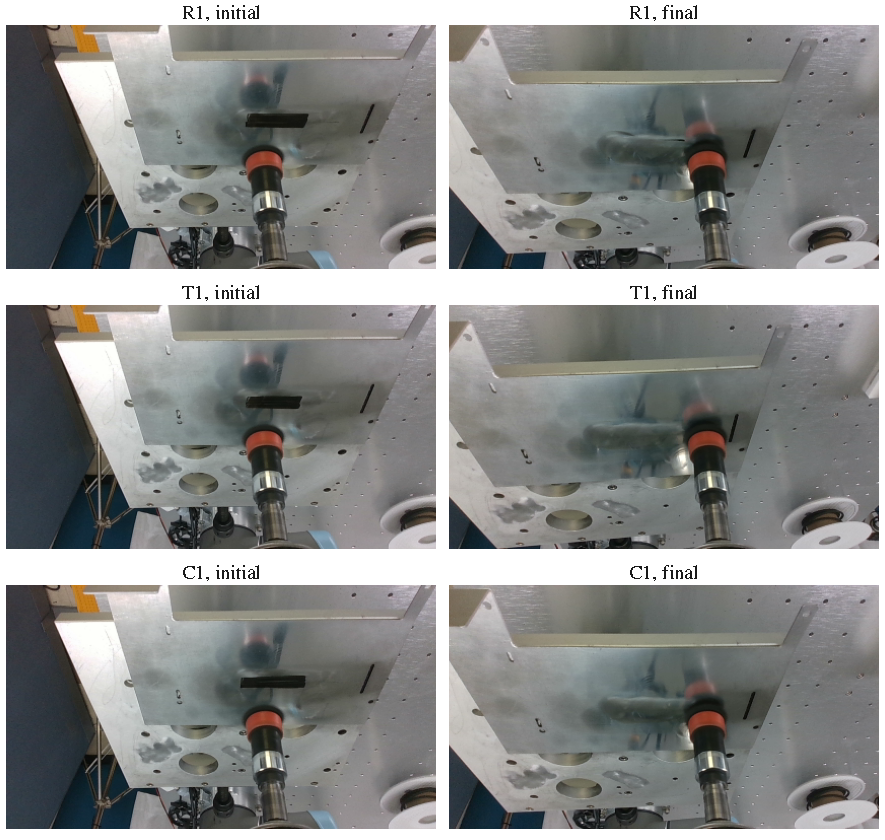
\includegraphics[width=.80\linewidth]{figures/e1_snapshot_panel.pdf}
\caption[First-run E1 initial and final snapshots]{Actual provider snapshots from the original E1 R1, T1, and C1 executions on 15 October 2026. Initial/final denote saved provider snapshots rather than matched metrology exposures; viewpoint, occlusion, and timing can differ. Visible marking changes do not measure scratch depth or surface restoration.}
\label{fig:e1_photos}
\end{figure}

Figure~\ref{fig:e2_sequence} presents uniformly sampled frames from the retained C1 video.

\figfull{e2_sequence.pdf}{Uniformly spaced camera-pane crops from the decodable portion of the first E2 C video. Only the adjacent diagnostic panel is omitted; camera overlays are retained. Times are video offsets, not synchronized stage-event times. The archived WebM ends prematurely and is not used to certify a complete exit sequence. A4 has no archived video.}{fig:e2_sequence}

\chapter{Additional R Diagnostic and E3 Image Archive}
\label{app:e3_archive}

\section{Additional R Executions and Source Precision}
Tables~\ref{tab:e1_rstar_all} and~\ref{tab:e1_rstar_ids} report the five additional outcomes and original identifiers.
\begin{table}[tbp]\centering\footnotesize
\caption[Additional R diagnostic runs]{All five \(R^{*}\) executions on 19 October, calculated from unrounded source CSVs and displayed to three decimals. The first diagnostic precedes four extension runs. These do not replace the original R1--R5. Time is first automatic procedure completion; pass speed uses the successful loaded-pass support.}
\label{tab:e1_rstar_all}\begin{tabular}{lrrrr}
\toprule
Run & Time (s) & $J_{\mathrm{excess}}$ (N\,s) & Peak (N) & Pass (mm/s) \\
\midrule
R$^{*}$1 & 22.481 & 0.000 & 21.488 & 10.696 \\
R$^{*}$2 & 25.319 & 0.000 & 22.000 & 10.887 \\
R$^{*}$3 & 25.520 & 0.000 & 20.541 & 10.886 \\
R$^{*}$4 & 25.458 & 0.000 & 22.727 & 10.822 \\
R$^{*}$5 & 25.420 & 0.000 & 20.944 & 10.915 \\
\bottomrule
\end{tabular}

\end{table}

The original per-run precision CSV and 17-page additional-R report describe the same five executions. Their identities, session/configuration identifiers, and template hashes are verified against the stored run contexts and input manifest. The first run uses configuration \path{e1ct_6c29a198a24df7a2}; repeats 2--5 use \path{e1ct_c5c424abc45fac4c}. All share the frozen template with SHA-256 prefix \texttt{1616a9f1bbb68df6}, the recorded feed, +18 N target, and v2 evaluator/observer. These identifiers preserve the one-then-four collection history.

\begin{table}[tbp]\centering\small
\caption[Original additional-R run identifiers]{Original identifiers for the additional \(R^{*}\) cohort. Full configuration and input hashes are supplied in the results manifest.}
\label{tab:e1_rstar_ids}\begin{tabular}{ll}
\toprule
Run & Original run identifier \\
\midrule
R$^{*}$1 & \texttt{E1\_CT\_NOMINAL\_R\_r1\_20261019T140517\_0921f1508b} \\
R$^{*}$2 & \texttt{E1\_CT\_NOMINAL\_R\_r2\_20261019T141109\_d8d222935d} \\
R$^{*}$3 & \texttt{E1\_CT\_NOMINAL\_R\_r3\_20261019T141211\_32499d64f6} \\
R$^{*}$4 & \texttt{E1\_CT\_NOMINAL\_R\_r4\_20261019T141312\_586a744e36} \\
R$^{*}$5 & \texttt{E1\_CT\_NOMINAL\_R\_r5\_20261019T141415\_bc2827864a} \\
\bottomrule
\end{tabular}

\end{table}

Reaggregation of the unrounded times gives \RstarTimeMeanPrecision~s and sample SD \RstarTimeSDPrecision~s, reproducing the displayed \EoneRstarTime\(\pm\)\EoneRstarTimeSD~s. The source-derived values and original identifiers are retained in \path{data/e1_rstar_source_runs.csv}. All five zero excess integrals and the shorter first run remain included.

\section{E3 Main-Run Pixel Areas}
Table~\ref{tab:e3_all_runs} lists the native-pixel areas for every main selected run.
\begin{table}[tbp]\centering\footnotesize
\caption[Individual E3 main-run image areas]{All 20 main selected N/P1/D1/D2 runs. Native-pixel areas are reproduced from the original RGB and frozen annotations and agree with the stored masks, CSVs, and image report. Percentages use Equation~\eqref{eq:e3_removal}. D1-4's final area and percentage remain null. Image evaluability is not procedure success.}
\label{tab:e3_all_runs}\begin{tabular}{lrrrl}
\toprule
Run & $A_{\mathrm{before}}$ (px) & $A_{\mathrm{after}}$ (px) & Removal (\%) & Note \\
\midrule
N-1 & 837 & 0 & 100.000 & image evaluable \\
N-2 & 879 & 0 & 100.000 & image evaluable \\
N-3 & 699 & 0 & 100.000 & image evaluable \\
N-4 & 697 & 0 & 100.000 & image evaluable \\
N-5 & 712 & 0 & 100.000 & image evaluable \\
P1-1 & 858 & 31 & 96.387 & image evaluable \\
P1-2 & 846 & 6 & 99.291 & image evaluable \\
P1-3 & 772 & 11 & 98.575 & image evaluable \\
P1-4 & 846 & 2 & 99.764 & image evaluable \\
P1-5 & 799 & 50 & 93.742 & image evaluable \\
D1-1 & 546 & 41 & 92.491 & image evaluable \\
D1-2 & 676 & 0 & 100.000 & image evaluable \\
D1-3 & 680 & 0 & 100.000 & image evaluable \\
D1-4 & 700 & \NA & \NA & tool occlusion \\
D1-5 & 798 & 0 & 100.000 & image evaluable \\
D2-1 & 768 & 79 & 89.714 & image evaluable \\
D2-2 & 738 & 13 & 98.238 & image evaluable \\
D2-3 & 794 & 128 & 83.879 & image evaluable \\
D2-4 & 743 & 13 & 98.250 & image evaluable \\
D2-5 & 684 & 12 & 98.246 & image evaluable \\
\bottomrule
\end{tabular}

\end{table}

The source-derived per-run identities and areas are captured in \path{data/e3_source_area_runs.csv}. Their ratios reproduce the reported main condition means and sample SDs. P1 ranges from 93.742 to 99.764\%, evaluable D1 from 92.491 to 100.000\%, and D2 from 83.879 to 98.250\%. The eight 100\% observations (five N and D1-2/3/5) mean black-ink nondetection under the established criterion. Figure~\ref{fig:e3_lowest_removal} preserves D2-3, the lowest observed individual removal, including all 128 residual pixels.

\begin{figure}[tbp]\centering
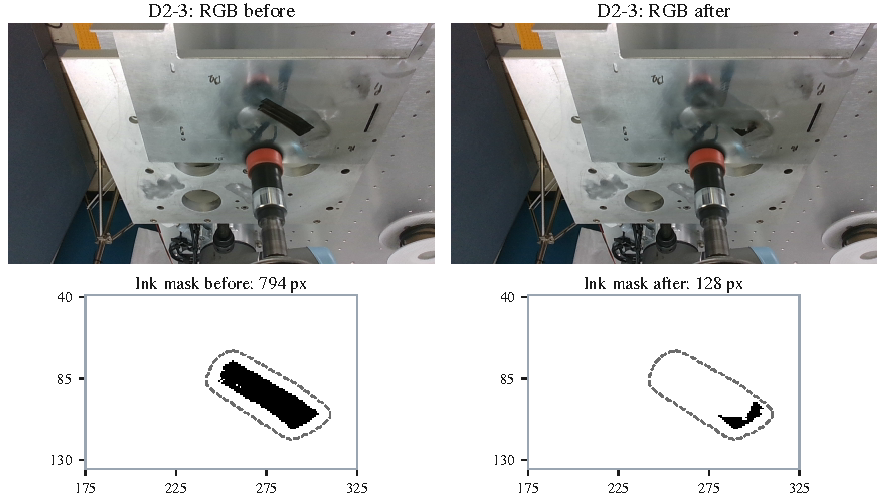
\includegraphics[width=\linewidth]{figures/e3_D2-3_native_evidence.pdf}
\caption[Lowest observed E3 removal, D2-3]{D2-3: original RGB and unchanged masks. The 794 initial and 128 residual pixels give 83.879\% removal. The common native-coordinate crop, dashed ROI, and black ink pixels follow the main evidence figures. This observed value is retained in D2's five-run mean.}
\label{fig:e3_lowest_removal}
\end{figure}

\section{Occlusion, Interruption, and P2 Exclusion}
Table~\ref{tab:e3_p2_archive} preserves the five excluded P2 image records. Figures~\ref{fig:e3_d1_occlusion} and~\ref{fig:e3_p2_occlusion} show the retained interruption and occlusion evidence.
\begin{table}[tbp]\centering\footnotesize
\caption[Executed P2 archive records]{P2 was executed five times and remains in the original 25-run selection. Every final photograph is tool-occluded. The initial areas are retained; whole-stain final areas and removal percentages are unavailable, not zero. P2 is outside the main four-condition removal evaluation.}
\label{tab:e3_p2_archive}\begin{tabular}{lrrl}
\toprule
Run & $A_{\mathrm{before}}$ (px) & Image result & Original stop \\
\midrule
P2-1 & 777 & unavailable & \texttt{operator\_finish} \\
P2-2 & 773 & unavailable & \texttt{operator\_finish} \\
P2-3 & 652 & unavailable & \texttt{operator\_finish} \\
P2-4 & 717 & unavailable & \texttt{operator\_finish} \\
P2-5 & 778 & unavailable & \texttt{operator\_finish} \\
\bottomrule
\end{tabular}

\end{table}

D1-4 retains \texttt{manual\_abort}; its interruption-time diagnostic frame contains visible residual marking and final tool occlusion. The report identifies the frame as received 34.5 ms before the abort request (source stamp approximately 0.55 s before it). No post-HOME photograph is available. The visible region is not used to estimate hidden total residual area. P2's initial frames are same-run pre-execution raw RGB, replacing initially occluded photographs; the final occlusion remains. These records are not removed or renamed in the archive.

\begin{figure}[tbp]\centering
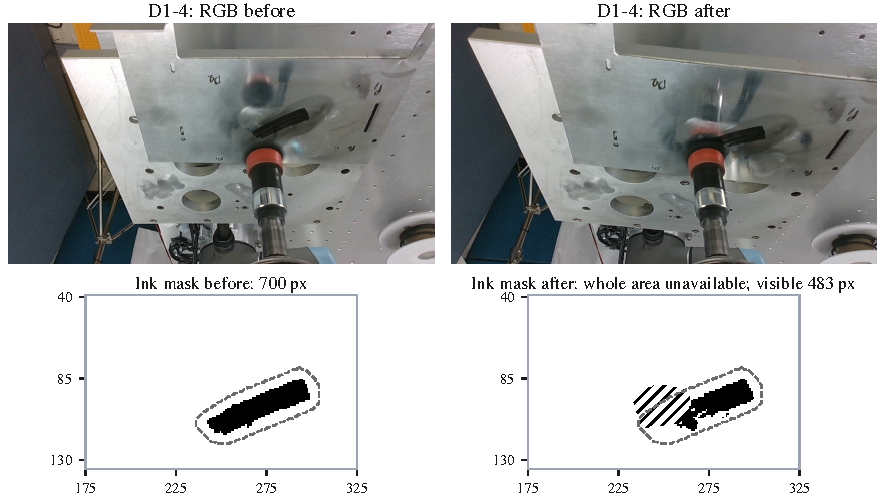
\includegraphics[width=\linewidth]{figures/e3_D1-4_native_evidence.pdf}
\caption[D1-4 retained interruption and occlusion evidence]{D1-4 original pre-task RGB and interruption-time diagnostic frame, with the unchanged saved masks. Hatching denotes final tool occlusion in the initial-frame reference grid. Visible residual ink is retained; hidden residual area is not estimated and whole-stain removal remains null. The existing surface-feature alignment is used for the occlusion display only.}
\label{fig:e3_d1_occlusion}
\end{figure}

\begin{figure}[tbp]\centering
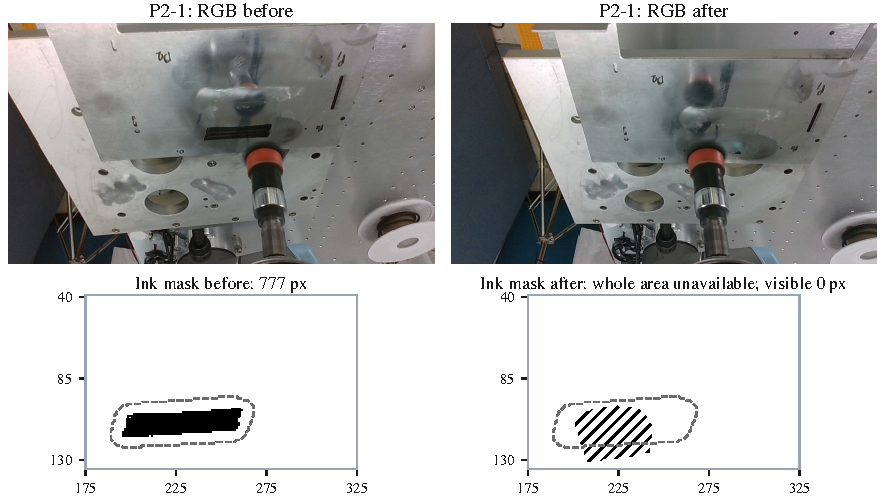
\includegraphics[width=\linewidth]{figures/e3_P2-1_native_evidence.pdf}
\caption[P2 retained final occlusion example]{P2-1 original pre-execution initial RGB and final image, with saved masks and occlusion hatching. The same-run initial replacement exposes the marking; final tool occlusion prevents whole-stain measurement. The mask display uses the established surface homography without reconstructing hidden image content. All five P2 records remain in the 25-run archive.}
\label{fig:e3_p2_occlusion}
\end{figure}

\section{Reused Segmentation Sensitivity and Procedure Diagnostics}
The report's sensitivity check keeps annotations and ROI fixed and changes the gray threshold equally in before/after images. Table~\ref{tab:e3_sensitivity} reproduces the published condition means at their printed precision; no new threshold or manual boundary is selected.

\begin{table}[tbp]\centering\small
\caption[Archived E3 threshold sensitivity]{Existing sensitivity results from the image report, p.36. Values are condition-mean percentages; main gray threshold is 45. These are not sample SD or confidence intervals. D1 uses four images throughout.}
\label{tab:e3_sensitivity}
\begin{tabular}{lrrr}\toprule
Condition & gray \(\leq40\) & gray \(\leq45\) & gray \(\leq50\) \\ \midrule
N & 100.000 & 100.000 & 100.000 \\
P1 & 97.912 & 97.552 & 96.914 \\
D1 & 98.124 & 98.123 & 98.056 \\
D2 & 94.659 & 93.665 & 92.932 \\
\bottomrule\end{tabular}
\end{table}

The archived v2 procedure outcomes are 8 completed and 17 \texttt{observation\_unavailable} in the original 25-run selection, with 24/25 HOME returns. The 25-page execution report, its per-run metrics CSV, and the selected run contexts retain these same identities and diagnostic labels. They are auxiliary procedure records on that archive, not removal successes or outcomes for the main 20-run subset. Image inclusion is independent of them; the force/path evaluator is not rerun for the image analysis.

\section{Evidence Availability and Reproduction}
The 39-page image report's pp.10--34 contain one RGB/ROI/mask evidence panel per selected run. The original \path{image_pair_manifest.json} and CSV, \path{analysis_config.json}, \path{annotations.json}, and \path{occluded_runs.csv} are linked to the frozen 25-run selection. All 50 original RGB files match the recorded file hashes. The saved per-run contexts confirm the registered offsets, common C checkpoint/normalizer identifiers, and condition-specific termination implementations.

Reprocessing the original RGB with the unchanged algorithm, inclusive gray threshold 45, and saved polygon/ROI settings reproduces all 25 initial areas, 19 available final areas, and visible-residual diagnostics for the six occluded cases. The 25 initial ink masks, 25 final aligned masks, and 25 initial ROI arrays are pixel-identical to their archived counterparts. All 19 evaluable pairs use verified identity surface registration. The six occluded pairs retain their original surface-feature alignment and unavailable whole-stain values. This is RGB-level computational reproduction, in addition to CSV aggregation and mask comparison; it is not an independent reassessment of the manual semantic labels.

The native figure assets preserve the original \(424\times240\) photographs. Binary-mask panels use the same \(x=175{:}325\), \(y=39{:}135\) crop and scale before/after and across displayed cases. Nearest-neighbor display preserves individual pixels; dashed vector ROI boundaries and occlusion hatching are annotations. No enhanced or generated photograph is used for measurement. The supplied display manifest records the selected original run IDs and hashes. Full source mapping, verification levels, software versions, and commands are supplied separately from the standalone document build.


\chapter{Development Extensions}
\label{app:development_extensions}

\section{Execution-Derived Dose}
\label{chap:removal_estimation}
The repository includes an execution-derived heatmap recorder. It integrates a Preston-style force--speed product along the measured path and optionally spreads it over a nominal tool kernel. Its diagnostic quantity can be expressed as
\begin{equation}
 D(x,y)=\sum_k\kappa\,F_{n,k}\,v_k\,\Delta t_k\,
                 K_{\mathrm{tool}}(x-x_k,y-y_k),
 \label{eq:preston_spatial}
\end{equation}
where \((x_k,y_k)\) is the recorded path location, \(F_{n,k}\) the implementation's selected force component or projection, \(v_k\) its selected speed, \(\Delta t_k\) the observation duration, and \(K_{\mathrm{tool}}\) a spatial spreading kernel. Without a measured coefficient and tool-response calibration, \(\kappa\) defines relative scale and \(D\) has arbitrary units. Different recorder/extension versions also make different kernel and speed-model choices.

Figure~\ref{fig:diagnostic_heatmap} illustrates this uncalibrated diagnostic quantity.

\begin{figure}[tbp]\centering
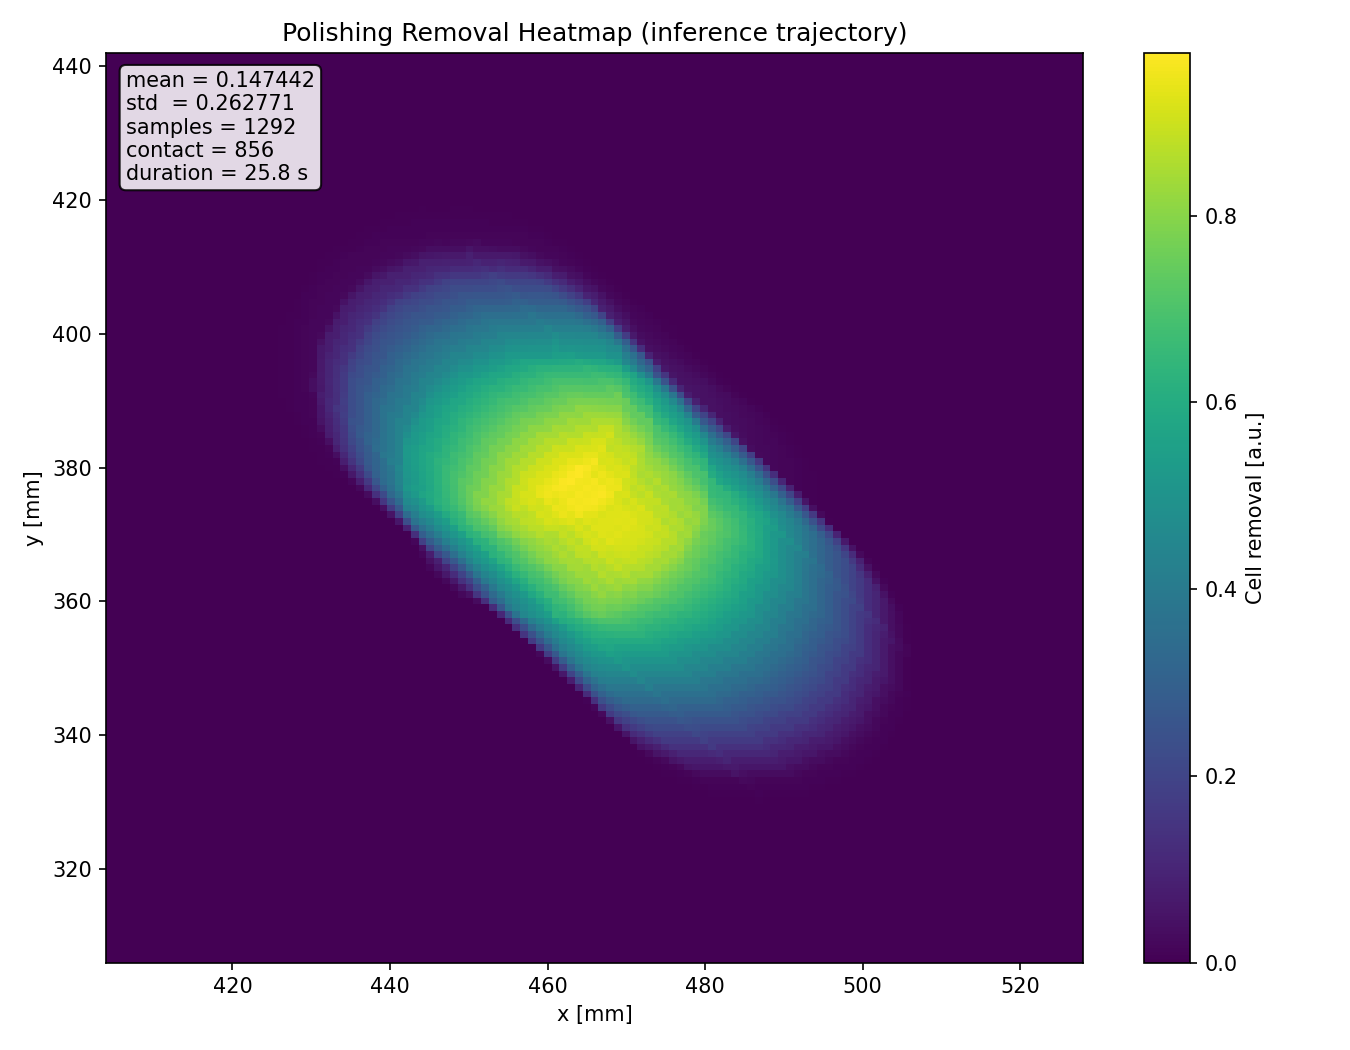
\includegraphics[width=\linewidth]{figures/E1_C1_diagnostic_heatmap.png}
\caption[Uncalibrated execution heatmap]{Historical execution-derived heatmap from E1 C1 on 14 October 2026, reproduced with its original axes and colorbar. Values are an uncalibrated model diagnostic in arbitrary units. They are not measured removal depth, effective contact footprint, or surface-quality improvement. This historical illustration is separate from the 15 October primary E1 cohort.}
\label{fig:diagnostic_heatmap}
\end{figure}

The implementation and generated artifact support calling this an implemented diagnostic extension. They do not support the older claim of a calibrated material-removal model. Its spatial distribution may help inspect where modeled processing exposure accumulated, but equal dose is not demonstrated equal removal on the actual specimen.

\section{Blending and Adaptive Execution Assets}
\label{chap:blending}
The project also contains finite local blending-path generation from an existing dose map, construction of an additional spatial target, and time allocation along a path. The 13 October extension prepares a sequence in which an initial skill is followed by a separate blending pass and diagnostic displays. Its archived validation includes offline planning from an earlier execution. That is evidence of an implemented extension, not an E1--E3 surface-uniformity result.

Separate 14 October adaptive-velocity records provide development experience with reference-clock progression and replanning. The located runtime files contain five online-OFF development attempts across multiple versions. Their completion status does not establish a controlled adaptive ON/OFF process-quality comparison. A later source revision addresses a recorded stalled reference-clock case, but its README explicitly distinguishes offline checking from a new physical run. These records are therefore kept outside the nominal E2 A/B/C cohort.

Table~\ref{tab:extension_status} distinguishes the supported status of each extension.

\begin{table}[tbp]\centering\small
\caption[Status of inherited extensions]{Status of inherited extensions relative to the main thesis evidence.}
\label{tab:extension_status}
\begin{tabularx}{\textwidth}{P{0.32\textwidth}X}
\toprule Asset & Supported status \\ \midrule
Execution heatmap & Implemented and generated from runs; uncalibrated arbitrary-unit diagnostic. \\
Finite blending planner & Implemented; archived offline planning and integration preparation. Surface-quality improvement not established by the main comparisons. \\
Adaptive reference-clock execution & Separate versioned development attempts and code; controlled ON/OFF outcome benefit not established. \\
High-level residual RL for curved-surface restoration & Planned extension; completed skill-level training and quality-grounded evaluation not established in the selected evidence. \\
\bottomrule
\end{tabularx}
\end{table}

Residual adjustments to orientation and feed velocity based on residual removal demand remain a planned extension. Existing low-level learned mass/damping control is a different asset and does not validate that proposed high-level policy. The core motion--force skill in this thesis does not require a removal estimator, blending planner, or residual RL stage to count as an executable system.


